\section{Main result: a resolution boundary in GIM}\label{sec:gim-results}

\subsection{Structure held constant}
The animal and plant nets reach 13 and 14 states, respectively. No place,
transition, arc, or initial marking changes across the three interfaces.
Native PN-GDDA is 0.9975846 throughout (0.9975175 with the independently
derived 576-orbit partition). This describes nearly identical selected local
wiring, not mechanistic identity or execution equivalence. Figure
\ref{fig:gim-interface} makes the comparison's biological assumptions and
computed outcomes visible together.

\begin{figure}[t]
\centering
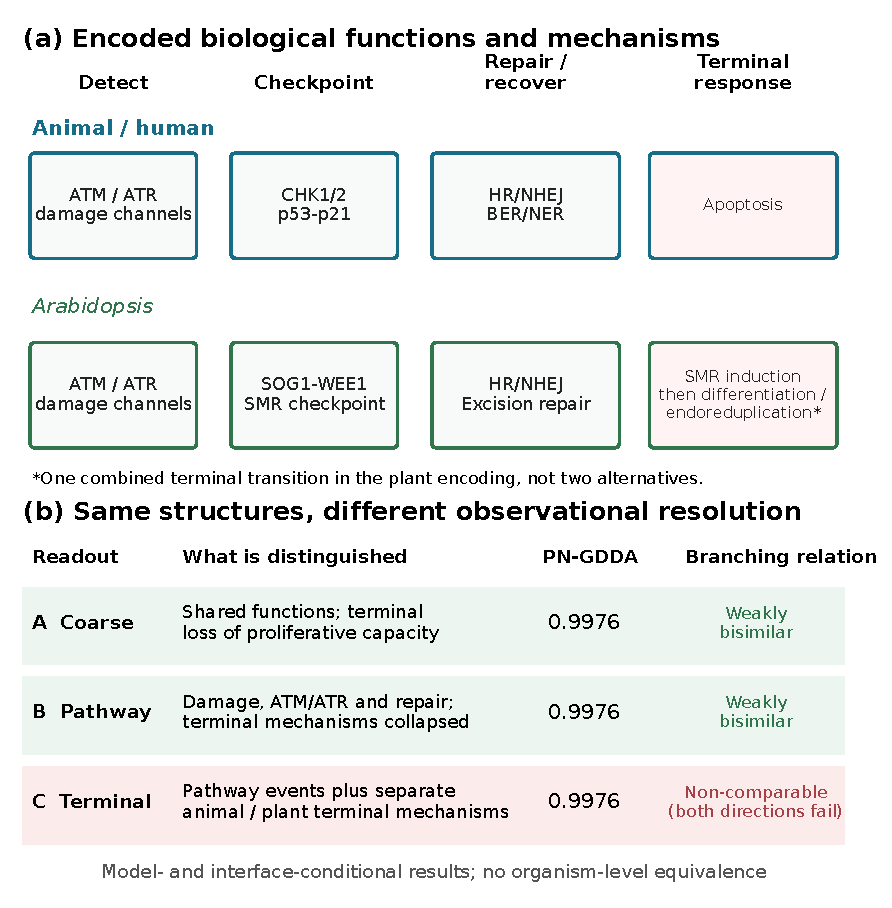
\includegraphics[width=\textwidth]{R2_Fig2.pdf}
\caption{Central GIM comparison. Upper-panel columns align encoded
animal/human and \tas{} functional categories; they are not a causal pathway
or a required sequence of outcomes. The lower panel
shows what each declared interface observes and the computed branching
relation. PN-GDDA remains 0.9976 because the structures are unchanged.
The combined plant terminal transition does not distinguish differentiation
from endoreduplication. Shared labels at A/B express a functional abstraction,
not identity between p53 and SOG1 or between terminal mechanisms.}
\label{fig:gim-interface}
\alttext{Animal and Arabidopsis damage-response functions above a three-row
interface comparison: A and B are weakly bisimilar; C is non-comparable,
with structural similarity constant at 0.9976.}
\end{figure}

\subsection{Coarse function retains correspondence}
At Interface A, every observable detection, checkpoint, repair, restoration,
or cycle-exit step in either executable model can be matched by the other,
with this matching preserved at the resulting states. Internal relays can
require different numbers of steps. Formally, the systems are weakly but not
strongly bisimilar. The result licenses comparison at the declared shared
functional level; it does not identify their molecular implementations.

\subsection{Pathway distinctions do not yet break the relation}
Interface B distinguishes damage channels, ATM/ATR-associated signaling, and
broad repair families. The models still match recursively when terminal
loss of proliferative capacity remains a common observation. Both simulation
directions and weak bisimilarity hold; strong bisimilarity does not.
Thus, among these encodings and interfaces, distinguishing those pathway
events alone is insufficient to eliminate the correspondence.

\subsection{Terminal mechanisms eliminate both directions}
At Interface C, mammalian \texttt{apoptosis} and plant
\texttt{smr\_induction} followed by
\texttt{differentiation\_or\_endoreduplication} become distinct observations.
Neither model can match all observable moves of the other, so weak
bisimilarity and both simulation directions fail. This is not an unexpected
biological discovery: the terminal labels intentionally encode prior knowledge
of different mechanisms. The computational result confirms where, in the
tested sequence of readouts, that distinction prevents recursive matching.
The depth-six trace distance becomes 0.3529 rather than zero; LTS-GDA changes
from 0.9508 to 0.8921. These diagnostics accompany the formal decision, not
replace it (Table~\ref{tab:gim-sensitivity}).

\begin{table}[t]
\tbl{Recomputed GIM results. Animal$\preceq$Plant means that the plant model
simulates the animal model; Plant$\preceq$Animal is the reverse.
Strong bisimilarity is false throughout.\label{tab:gim-sensitivity}}{
\begin{tabular}{@{}lccp{1.10in}rr@{}}
\toprule
Interface & Animal$\preceq$Plant & Plant$\preceq$Animal & Class & $d_6$ & PN-GDDA\\
\colrule
A: coarse & Y & Y & weak bisimulation & 0.0000 & 0.9976\\
B: pathway & Y & Y & weak bisimulation & 0.0000 & 0.9976\\
C: terminal & N & N & non-comparable & 0.3529 & 0.9976\\
\botrule
\end{tabular}}
\end{table}

\subsection{What changes when observability changes?}
Interfaces A and B aggregate terminal mechanisms into a shared functional
readout, whereas C separates them. The observed boundary is therefore
\emph{between B and C within this declared interface family}, not a uniquely
identified or globally minimal biological resolution. There is no exhaustive
search over all possible interfaces, and no experimental threshold is inferred.
The constant structural score isolates observability from topological change.

Prior biology supplies the distinct terminal mechanisms; PN-GDDA describes
their selected wiring; the executable comparison determines whether a
recursive correspondence survives each declared readout. Whether such a
model-level boundary predicts a cross-species experimental boundary remains
unvalidated. One testable interpretation is that readouts aggregating terminal
loss of proliferative capacity may preserve an apparent correspondence that
mechanism-specific readouts do not. This is a model-derived hypothesis, not an
assay result. The full Petri nets remain in \ref{app:gim-nets}.
